\section{Outer loop projected gradient descent}
\label{sec:outer_loop_pgd}

The density estimation framework formulated in Section~\ref{sec:constrained_optimisation} requires the minimisation of the convex empirical objective $f(\cdot)$ defined in \eqref{eq:finite_objective}, subject to the polyhedral feasible set $\mathcal{H}$ defined in \eqref{eq:polyhedral_set}. To navigate this constrained polynomial coefficient space and compute the optimal transport map, we deploy a PGD architecture. The PGD algorithm operates an outer learning loop, indexed by $t$, which iteratively updates the decision variables governing the map. Each outer iteration comprises two sequential mathematical operations: an unconstrained descent step evaluated over the target distribution, followed by an exact Euclidean projection to enforce physical monotonicity. 

In the first operation, we compute the gradient of the objective function evaluated at the current feasible iterate, $\nabla f(w^{(t)})$. The algorithm takes an unconstrained step in the direction of the negative gradient, scaled by a \emph{step size} (or \emph{learning rate}) parameter $\eta^{(t)}$. This operation produces an intermediate, potentially infeasible coefficient vector $w^{\circ}$:
\begin{equation}
    w^{\circ} = w^{(t)} - \eta^{(t)} \nabla f(w^{(t)}).
    \label{eq:pgd_unconstrained_gradient_step}
\end{equation}

The learning rate schedule follows an inverse time decay model $\eta^{(t)} = \eta^\circ / (1 + \gamma t)$, where $\eta^\circ \in \mathbb{R}$ is the initial learning rate and $\gamma \in \mathbb{R}$ is a decay coefficient. This decay mechanism helps the optimiser settle into narrow minima as the gradients decrease in magnitude during later iterations. This inverse model is visualised in Figure~\ref{fig:learning_rate_decay}, evaluated with an initial learning rate of $\eta^\circ = 0.1$ across varying decay coefficients $\gamma$.

\begin{figure}[htpb]
    \centering
    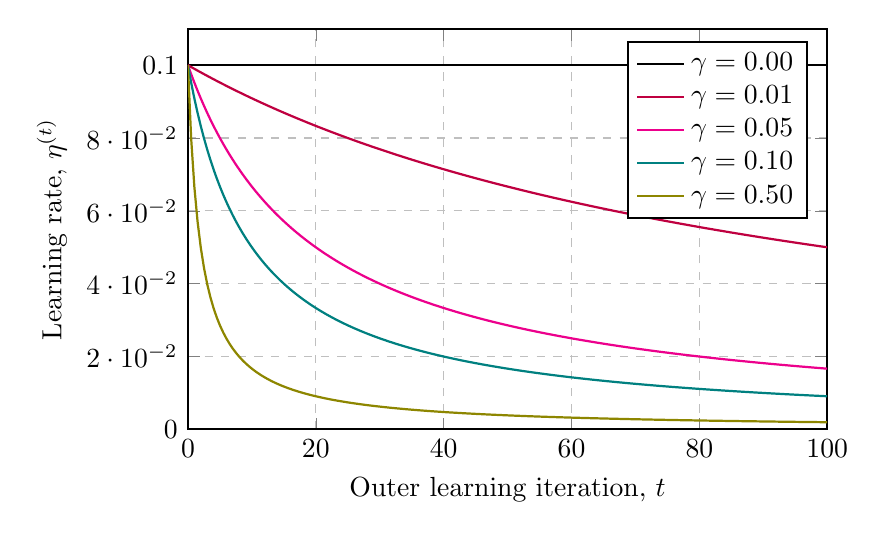
\begin{tikzpicture}
        \begin{axis}[
            width=0.8\textwidth,
            height=0.55\textwidth,
            xlabel={Outer learning iteration, $t$},
            ylabel={Learning rate, $\eta^{(t)}$},
            xmin=0, xmax=100,
            ymin=0, ymax=0.11,
            grid=major,
            grid style={dashed, gray!50},
            legend pos=north east,
            legend cell align={left},
            thick
        ]
        
        \addplot[domain=0:100, samples=200, color=black] {0.1 / (1 + 0*x)};
        \addlegendentry{$\gamma = 0.00$}
        
        \addplot[domain=0:100, samples=200, color=purple] {0.1 / (1 + 0.01*x)};
        \addlegendentry{$\gamma = 0.01$}
        
        \addplot[domain=0:100, samples=200, color=magenta] {0.1 / (1 + 0.05*x)};
        \addlegendentry{$\gamma = 0.05$}
        
        \addplot[domain=0:100, samples=200, color=teal] {0.1 / (1 + 0.1*x)};
        \addlegendentry{$\gamma = 0.10$}
        
        \addplot[domain=0:100, samples=200, color=olive] {0.1 / (1 + 0.5*x)};
        \addlegendentry{$\gamma = 0.50$}
        
        \end{axis}
    \end{tikzpicture}
    \caption{Inverse time decay schedule for the unconstrained learning rate.}
    \label{fig:learning_rate_decay}
\end{figure}
The selection of the decay coefficient $\gamma$ strictly governs the exploration-exploitation trade-off during the unconstrained descent phase. A value of $\gamma = 0$ reduces the schedule to a constant learning rate. While a constant step size promotes continuous exploration of the objective landscape, it frequently induces numerical oscillations around the optimal parameters and prevents the algorithm from converging to a precise local minimum. Conversely, an aggressive decay rate (e.g., $\gamma \ge 0.1$) rapidly diminishes the step size. This forces the optimiser to exploit the local geometry and settle quickly, but risks premature convergence to shallow, sub-optimal minima if deployed before the iterates reach the primary basin of attraction. A moderate decay provides a structural balance, allowing the framework to traverse flat ravines during the early learning iterations while ensuring the step size becomes sufficiently small to satisfy strict polyhedral feasibility constraints as $t$ approaches $T-1$.

Because this unconstrained step is driven solely by the maximum likelihood objective, it does not guarantee adherence to the structural constraints. The intermediate vector $w^{\circ}$ will frequently exit the feasible polyhedral intersection $\mathcal{H}$, corresponding to a transport map that temporarily violates the monotonicity requirement.

To rectify this and ensure the map remains strictly monotonic at every learning iteration, the second operation requires projecting $w^{\circ}$ back onto $\mathcal{H}$. This requires finding the unique feasible point that minimises the Euclidean distance to $w^{\circ}$, which is mathematically equivalent to solving the CQP defined in \eqref{eq:cqp_projection}. We denote the exact Euclidean projection operator onto the set $\mathcal{H}$ as $\mathcal{P}_{\mathcal{H}}(\cdot)$. The projected point becomes the feasible update for the subsequent learning iteration:
\begin{equation}
    w^{(t+1)} = \mathcal{P}_{\mathcal{H}}(w^\circ).
    \label{eq:pgd_projection_step}
\end{equation}

Within this framework, the evaluation of the projection operator $\mathcal{P}_{\mathcal{H}}(\cdot)$ acts as a direct function call to the accelerated Dykstra algorithm developed in Chapter~\ref{ch:dykstra}. The integration of the inner projection solver with this outer learning loop, including the dynamic parameterisation of the projection iteration limits and other computational optimisation techniques adopted, is detailed further in Section~\ref{sec:inner_loop_integration}.

The backbone of our PGD implementation therefore consists of applying the unconstrained gradient descent update~\eqref{eq:pgd_unconstrained_gradient_step} followed by the projection step~\eqref{eq:pgd_projection_step}. However, evaluating the deterministic gradient over the complete particle set at every iteration is computationally expensive and leaves the optimiser susceptible to ``slowing down'' in flat ravines within the objective landscape. To address these limitations and scale the framework, we replace the full-batch gradient evaluation with a stochastic approximation.